%%%%%%%%%%%%%%%%%%%%%%%%%%%%%%%%%%%%%%%%%%%%%%%%%%%%%%%%%%%%%%%%%%%%%%%%%%%%%%%%
\section{User API} \label{UserAPI}
%%%%%%%%%%%%%%%%%%%%%%%%%%%%%%%%%%%%%%%%%%%%%%%%%%%%%%%%%%%%%%%%%%%%%%%%%%%%%%%%

%===============================================================================
\subsection{IntensityData}
%===============================================================================

The \Code{IntensityData} object stores the
simulated or real intensity data together with the axes definition of the detector in BornAgain's internal format.
During the simulation setup
it is created automatically when the user specifies the detector characteristics and is filled with the simulated intensities after the simulation is completed.

\begin{lstlisting}[language=python, style=eclipseboxed]
simulation = Simulation()
simulation.setDetectorParameters(10, -5.0*degree, 5.0*degree, 5, 0.0*degree, 1.0*degree)
...
simulation.runSimulation()
intensity = simulation.getIntensityData() @\label{py:UserApi:intensity}@
\end{lstlisting}

The \Code{IntensityData} object retrieved in line~\ref{py:UserApi:intensity} corresponds to
the two dimensional detector pixel array as shown in \cref{fig:UserApi:IntensityData}.

\begin{figure}[ht]
  \centering
    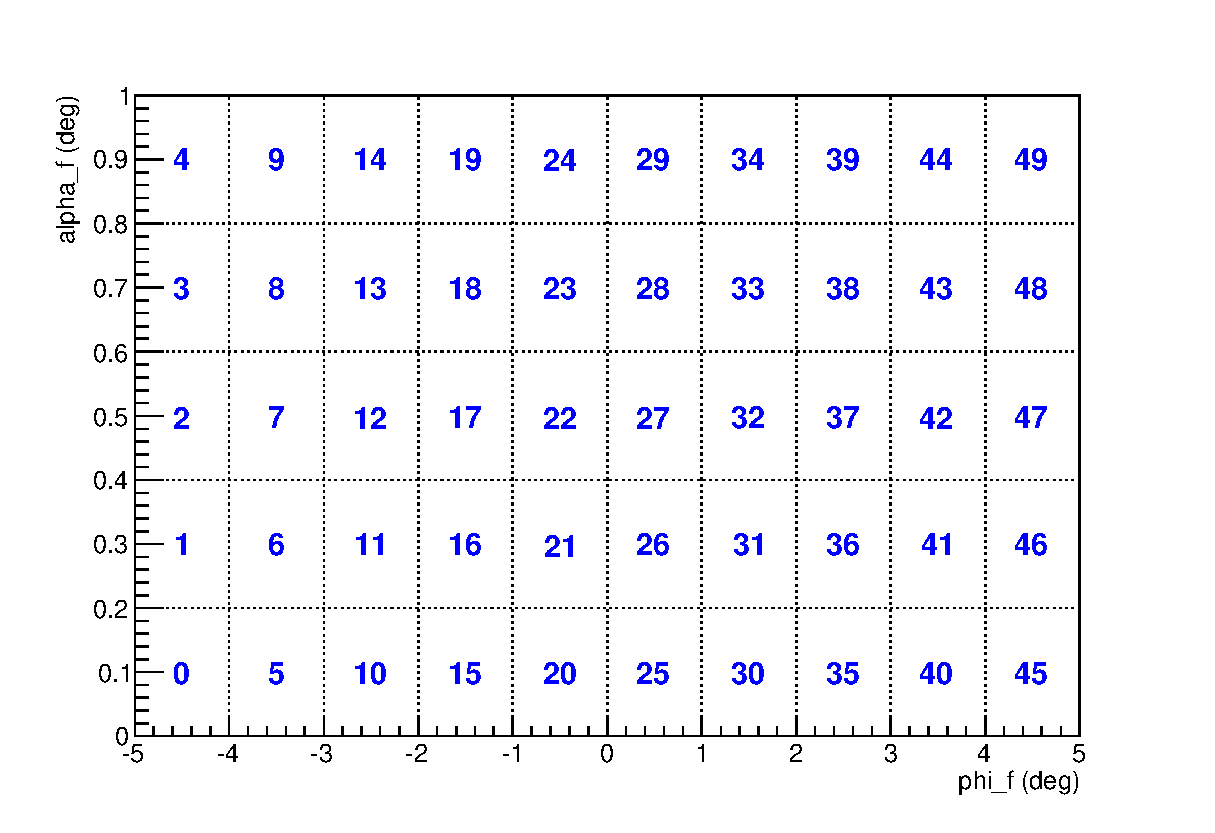
\includegraphics[clip=, width=120mm]{fig/drawing/UserAPI_IntensityDataLayout.eps}
  \caption{The axes layout of IntensityData object.}
  \label{fig:UserApi:IntensityData}
\end{figure}

The x-axis and y-axis of the figure correspond to the $\phi_f$ and $\alpha_f$ axes of the detector.
The x-axis is divided into 10 bins,
with low edge of the first bin set to $-5.0\,{\rm deg}$ and upper edge of the last bin set to $+5.0\,{\rm deg}$.
The y-axis is divided into 5 bins,
with low edge of the first bin set to $0.0\,{\rm deg}$ and upper edge of the last bin set to $1.0\,{\rm deg}$.
There are 50 bins in total (they are marked on the plot with indexes from 0 to 49), each bin will contain one intensity value.

During a standard simulation (i.e. no Monte-Carlo integration involved) intensities are calculated for $\phi_f, \alpha_f$ values corresponding to the bin centers, e.g. the intensity stored in bin\#42 will correspond to $\phi_f=3.5\,{\rm deg}, \alpha_f=0.5\,{\rm deg}$.
\vspace*{2mm}


\Note{
The \Code{IntensityData} object is not intended for direct usage from Python API. The idea is
that the API provides the user with the possibility to export the data from BornAgain internal format to the format of his choice as well as import user's data into BornAgain.
For the moment this functionality is limited to a few options explained below.
We encourage users feedback to implement the support of most requested formats.}


\subsubsection{Import/export of intensity data}
For the moment we provide following options:
\begin{itemize}
\item Import/export of \Code{IntensityData} object from/to \Code{numpy} array.
\item Import/export of \Code{IntensityData} object from/to text file.

\end{itemize}

\paragraph{Export to numpy array}

To export intensity data into  \Code{numpy} array the method \Code{getArray()} should be used
on \Code{IntensityData} object as shown in line \ref{py:UserApi:getArray} of
following code snippet.

\begin{lstlisting}[language=python, style=eclipseboxed]
intensity = simulation.getIntensityData()
array = intensity.getArray() @\label{py:UserApi:getArray}@
...
pylab.imshow(numpy.rot90(array, 1)) @\label{py:UserApi:imshow}@
pylab.show()
\end{lstlisting}

For the detector settings defined in the previous paragraph the dimensions of the resulting array will be (10,5). By using \Code{numpy} indexes the user can get access to the intensity values, e.g.
\Code{array[0][0]} corresponds to the intensity in bin\#0 of \cref{fig:UserApi:IntensityData},
\Code{array[0][4]} to bin\#4,
\Code{array[1][0]} to bin\#5,
\Code{array[8][2]} to bin\#42,
\Code{array[9][4]} to bin\#49.


To plot this resulting numpy array with \Code{matplotlib} it has to be rotated counter-clockwise
to match \Code{matplotlib} conventions as shown in line~\ref{py:UserApi:imshow}.


%\subsubsection{Direct access to the data}
%User can access to the

%\begin{lstlisting}[language=python, style=eclipseboxed]
%for i in range(0, intensity.getAllocatedSize()):
%    print intensity[i]
%\end{lstlisting}


\subsubsection{Importing from numpy array}

To use fitting the user has to load experimental data into BornAgain fitting kernel.
To read experimental data the user has to create
IntensityData object, fill it with the experimental  intensity values and pass
this object to the fitting kernel.

First, the user creates empty \Code{IntensityData} as shown
in line~\ref{py:UserApi:IntensityData} of the following code snippet.
\begin{lstlisting}[language=python, style=eclipseboxed]
data = IntensityData() @\label{py:UserApi:IntensityData}@
data.addAxis(FixedBinAxis("phi_f", 10, -5.0*degree, 5.0*degree)) @\label{py:UserApi:phi_f}@
data.addAxis(FixedBinAxis("alpha_f", 5, 0.0*degree, 1.0*degree)) @\label{py:UserApi:alpha_f}@
...
array = numpy.zeros((10, 5)) # fill array with experimental intensities @\label{py:UserApi:create_array}@
...
data.setRawDataVector(array.flatten().tolist()) @\label{py:UserApi:set_raw}@

fitSuite = FitSuite() @\label{py:UserApi:fit_suite}@
fitSuite.addSimulationAndRealData(simulation, data) @\label{py:UserApi:add_real_data}@
\end{lstlisting}

In lines~\ref{py:UserApi:phi_f}, \ref{py:UserApi:alpha_f} two axes with fixed bin sizes
are defined to represent the detector layout as shown in \cref{fig:UserApi:IntensityData}.
The constructor of \Code{FixedBinAxis} object has the following signature

\begin{lstlisting}[language=python, style=eclipse,numbers=none]
FixedBinAxis(title, nbins, min_angle, max_angle)
\end{lstlisting}

The created \Code{IntensityData} object has to be filled with experimental intensities
using \Code{numpy} array prepared by the user (lines ~\ref{py:UserApi:create_array}-~\ref{py:UserApi:set_raw}). In lines \ref{py:UserApi:fit_suite},\ref{py:UserApi:add_real_data} the fitting kernel is created and initialized with \Code{Simulation} object and
\Code{IntensityData} object representing the experimental data.


\subsubsection{Saving intensity data to text file.}

The special class \Code{IntensityDataIOFactory} is intended for saving the intensity data
in different datafile formats. For the moment, it only supports saving the data in specific BornAgain's text files (the file extention \Code{*.int}).

\begin{lstlisting}[language=python, style=eclipseboxed]
intensity = simulation.getIntensityData()
IntensityDataIOFactory.writeIntensityData(intensity, 'file_name.int')
\end{lstlisting}

\subsubsection{Reading intensity data from a text file.}
The same class is also intended for reading intensity data
from files with different formats. For the moment, it only supports reading the data from text files of special BornAgain's format (the file extention \Code{*.int}).

\begin{lstlisting}[language=python, style=eclipseboxed]
intensity = IntensityDataIOFactory.readIntensityData('file_name.int')
\end{lstlisting}
